\chapter{Architecture} \label{chapter5}

In this chapter, we will be discussing the technologies we chose to use for this project and our implementation.

\section{Mobile technology} \label{5:technology}

\subsection{The native approach} \label{5:technology_native}

In terms of the best core technology/language to use for the mobile application itself, we initially considered a native Android solution, since the vast majority of students in the faculty (80\% according to our study, section \ref{3:target_audience}) own an Android phone. However, since our application should be available to all students, and the quality of information is dependent on the number of users in a collaborative system, a pure Android solution proved not to be the best approach.

Native mobile implementations come with various benefits, from consistent, native-compliant application design (see appendix \ref{a:native_cross}) to outstanding performance and making the best of what the device has to offer. However, having only one supported platform would mean excluding a significant number of students from the user base. On the other hand, having two separate, native implementations for each mobile OS (one written in Java/Kotlin for Android, and one written in Objective-C/Swift for iOS) would require double the amount of time and effort. Due to the complexity of the application, the native approach is regrettably out of the question.

\subsection{The cross-platform approach} \label{5:technology_cross}

Given the circumstances, we decided to look into cross-platform technologies for mobile applications. According to Sandeep Agarwal\cite{agarwal2019best}, the 5 most popular mobile app development frameworks in 2019 are React Native\footnote{https://reactnative.dev/} (by Facebook), \gls{flutter}\footnote{https://flutter.dev/} (by Google), Ionic\footnote{https://ionicframework.com/} (by Drifty), Xamarin\footnote{https://dotnet.microsoft.com/apps/xamarin} (by Microsoft) and PhoneGap\footnote{https://phonegap.com/} (by Adobe). Due to our developer not having any prior experience with JavaScript development, we decided to choose between \gls{flutter} and Xamarin. This decision is mainly influenced by the other three frameworks all being based on HTML5, CSS, and JavaScript. In terms of development language, Xamarin uses C\# and .NET, while \gls{flutter} uses Dart.

Both \gls{flutter} and Xamarin have the significant benefit of being part of a vast development ecosystem, therefore choosing the technology also implies choosing the ecosystem. \gls{flutter} is integrated within the Google ecosystem (including support for services like Google Cloud\footnote{https://cloud.google.com/} and a designated development environment: Android Studio\footnote{https://developer.android.com/studio/}). Xamarin is part of the Microsoft ecosystem (offering alternatives such as Azure Cloud Services\footnote{https://azure.microsoft.com/en-in/services/cloud-services/} and Visual Studio\footnote{https://visualstudio.microsoft.com/}).

Xamarin is a more "mature" framework with deep roots in the developer community since it was released in 2011, six years before \gls{flutter} came into the cross-platform market. However, \gls{flutter}'s community is growing rapidly, and the developers' response is overwhelmingly positive. According to the 2020 StackOverflow Developer Survey\cite{stackoverflow2020survey}, \gls{flutter} was rated the third most loved non-web framework and is the first mobile development framework in the list (with the second being React Native, and the third Xamarin).

Even though Xamarin provides support for more platforms (iOS, Android, Windows, macOS), it still requires platform-specific code for iOS and Android. For our use case (a mobile application), \gls{flutter} seems to be more appropriate since it provides better code reusability. The stable release of \gls{flutter} supports iOS and Android, while the beta and alpha channels provide web support and macOS support, respectively. A web version of a \gls{flutter} application can be run on any web-enabled device (including Windows and Linux devices, for which native support is still under development). Therefore we believe that \gls{flutter} appropriately meets the need for our application to be readily available for any student.

Upon careful consideration of the leading cross-platform technologies available for developing mobile applications, we have concluded that \textbf{\gls{flutter}} is the best technology for our application.

\section{Database} \label{5:database}

Being part of the Google ecosystem, \gls{flutter} offers seamless integration with the Google Cloud Platform and other Google services such as \gls{firebase}\footnote{https://firebase.google.com/}. For mobile applications, \gls{firebase} offers features such as analytics, database, and authentication, therefore we have decided to take advantage of it for all of our cloud-based needs.

\subsection{Firestore} \label{5:firestore}
Cloud Firestore\footnote{https://firebase.google.com/docs/firestore/} is a \gls{nosql} database that organises its data in \textit{collections} and \textit{documents}.

\subsubsection{Data model} \label{5:firestore_data_model}
\textbf{Collections} are simply a list of documents, where each document has an ID within the collection.

\textbf{Documents} are similar to a \gls{json} file, in that they contain different fields which have three important components: a \textit{name} - what we use to refer to the field, similar to a dictionary key -, a \textit{type} (which can be one of \mintinline{text}{string}, \mintinline{text}{number}, \mintinline{text}{boolean}, \mintinline{text}{map}, \mintinline{text}{array}, \mintinline{text}{null}, \mintinline{text}{timestamp}, \mintinline{text}{geopoint}, \mintinline{text}{reference}), and the actual \textit{value}, the data contained in the field.
In addition to fields, documents can contain collections, which in turn contain other documents, thus allowing us to create a hierarchical structure within the database.

\subsubsection{Security} \label{5:firestore_security}
Firestore allows for defining specific security rules for each collection. Rules can be applied for each different type of transaction - \mintinline{text}{read}s (where single-document reads - \mintinline{text}{get} - and queries - \mintinline{text}{list} - can have different rules) and \mintinline{text}{write}s (where \mintinline{text}{create}, \mintinline{text}{delete} and \mintinline{text}{update} can be treated separately).

\subsection{Authentication} \label{5:authentication}
\gls{firebase} provides an entire suite of back-end services and \acrshort{sdk}s for authenticating users within an application, through FirebaseAuth\footnote{https://firebase.google.com/docs/auth}.

For our application, we use the following features:
\begin{itemize}
    \setlength{\topsep}{0.5pt}
    \setlength{\itemsep}{0.5pt}
    \setlength{\parsep}{0.5pt}
    \item account creation
    \item login
    \item password reset via e-mail
    \item account verification via e-mail
    \item account deletion
\end{itemize}

The class structure can be seen in appendix \ref{a:uml}, figure \ref{a:fig:uml_authentication}. The \mintinline{dart}{AuthProvider} class is responsible for communicating with FirebaseAuth.

This service automatically handles the authentication tokens and enforces security rules, which is particularly useful for an open-source application which users can fiddle with, such as ours. For example, multiple failed authentication attempts lead to a temporary timeout, and a user cannot delete their account unless they have logged in very recently (or refreshed their authentication token).

Firestore security rules (see subsection \ref{5:firestore_security}) can be enforced based on the user's \acrshort{uid}. This method means that, even though users can access the database connection string through the public repository, they can only do a limited set of actions on the database, depending on whether they are authenticated and their rights.

\subsection{Project database structure} \label{5:database_project}
We opted for a database architecture where all documents within a collection can contain a subset of fields from a given list, similar to a relational database table. Some fields are required to be present (similar to \mintinline{sql}{NOT NULL} columns in a \textit{SQL} database), while others might not be present (similar to a column with the \mintinline{sql}{NULL} property). This structure makes it easier to migrate to a relational database in the future, should the need arise.

The project database contains the following collections:

~

\faDatabase \hspace{0.1cm} \textbf{\mintinline{text}{users}}

This collection stores per-user data. The document key is the user's \mintinline{text}{uid} (from FirebaseAuth, see subsection \ref{5:authentication}).

All the documents in the collection share the structure described in table \ref{5:tab:users}.

\begin{table}[th]\small\linespread{1}
\caption{\textbf{users} collection structure}
\label{5:tab:users}
\begin{tabular}{| l | l | c | p{4.7cm} |}
\hline
\textbf{Field} & \textbf{Type} & \textbf{Required?} & \textbf{Additional info} \\
\hline
group & \mintinline{text}{string} & \Checkedbox & e.g. "314CB" 
\\
\hline
name & \mintinline{text}{map<string, string>} & \Checkedbox & keys are "first" and "last"
\\
\hline
permissionLevel & \mintinline{text}{number} & \CrossedBox & a numeric value that defines what the user is allowed to do; if missing, it is treated as being equal to zero
\\
\hline
\end{tabular}
\end{table}

A user can define their private events and websites, that only they can access. These will reside in the \textbf{events} and \textbf{websites} sub-collections, respectively, which have a similar structure as the root-level collections with the same names, described below in this section.

We define special \textit{\textbf{rules}} (see subsection \ref{5:firestore_security}) for this collection and its subcollections. Anyone can create a new user (a new document in this collection) if the \textit{permissionLevel} of the created user is \mintinline{text}{0}, \mintinline{text}{null} or not set at all. Authenticated users can only \mintinline{text}{read}, \mintinline{text}{delete} and \mintinline{text}{update} their own document (including its subcollections) and no one else's. However, they cannot modify the \textit{permissionLevel} field.

\clearpage

\faDatabase \hspace{0.1cm} \textbf{\mintinline{text}{websites}}

This collection stores useful websites, shown in the app under the \textbf{Portal} page. Which students they are relevant for depends on the \textit{degree} and \textit{relevance} fields (for more information, see the \textbf{filters} collection described below in this section).

The documents in this collection share the structure pictured in table \ref{5:tab:websites}.

\begin{table}[th]\small\linespread{1}
\caption{\textbf{websites} collection structure}
\label{5:tab:websites}
\begin{tabular}{| l | p{2.6cm} | c | p{7.1cm} |}
\hline
\textbf{Field} & \textbf{Type} & \textbf{Required?} & \textbf{Additional info} \\
\hline
category & \mintinline{text}{string} & \Checkedbox & one of: “learning”, “association”, “administrative”, “resource”, “other”
\\
\hline
degree & \mintinline{text}{string} &    \HollowBox & “BSc” or “MSc”, must be specified if \textit{relevance} is not \mintinline{text}{null}
\\
\hline
editedBy & \mintinline{text}{array<string>} & \CrossedBox & list of user IDs
\\
\hline
icon & \mintinline{text}{string} & \CrossedBox & path in Firebase Storage; if missing, it defaults to "icons/websites/globe.png"
\\
\hline
label & \mintinline{text}{string} & \Checkedbox & unless specified, the app sets this to be the link without the protocol
\\
\hline
link & \mintinline{text}{string} & \Checkedbox & it needs to include the protocol (\textit{http://}, \textit{https://} etc.)
\\
\hline
relevance & \mintinline{text}{null} /

\mintinline{text}{list<string>}& \Checkedbox & \mintinline{text}{null}\footnotemark if relevant for everyone, otherwise a string of filter node names
\\
\hline
\end{tabular}
\end{table}

\footnotetext{In Firestore, \mintinline{text}{null} is a data type; a field that is \mintinline{text}{null} is different from a field that is not present in a document.}

This collection also has a special set of \textbf{rules}\textit{} (see subsection \ref{5:firestore_security}), based on the permission levels described in section \ref{4:permissions_levels}. Since websites in this collection are public information (anyone can \mintinline{text}{read}), altering and adding data here is a privilege and needs to be monitored, therefore anyone who wants to modify this data needs to be authenticated in the first place. Users can \mintinline{text}{create} a new public website only if their \textit{permissionLevel} is equal to or greater than two  and they sign the data by putting their \textit{uid} in the \textit{addedBy} field. Users can \mintinline{text}{update} a website if they do not modify the \textit{addedBy} field and they sign the modification by adding their \textit{uid} at the end of the \textit{editedBy} list. Users can only delete a website if they are the ones who created it (their \textit{uid} is equal to the addedBy field) or if their \textit{permissionLevel} is equal to or greater than three.

\clearpage

\faDatabase \hspace{0.1cm} \textbf{\mintinline{text}{filters}}

This collection stores \mintinline{dart}{Filter} objects. These are essentially trees with named nodes and levels. In the case of the relevance filter, they are meant to represent the way the University organizes students:

\begin{minted}{text}
                              All
                _______________|______________
              /                                \
            BSc                               MSc // Degree
     ________|________                 ________|__ ...
   /                  \              /     |
  IS                 CTI            IA   SPRC ... // Specialization
..|..           ______|______       ⋮      ⋮
              /    |     |   \
           CTI-1 CTI-2 CTI-3 CTI-4                // Year
              ⋮    ⋮   __|... ⋮
                    /   |
                 3-CA 3-CB ...                    // Series
                 __|...
               /   |
           331CA 332CA ...                        // Group
\end{minted}

The tree-based structure is defined using \mintinline{text}{map}s, as pictured in table \ref{5:tab:filters}.

\begin{table}[th]\small\linespread{1}
\caption{\textbf{filters} collection structure}
\label{5:tab:filters}
\begin{tabular}{| l | p{2.6cm} | c | p{7.1cm} |}
\hline
\textbf{Field} & \textbf{Type} & \textbf{Required?} & \textbf{Additional info} \\
\hline
levelNames & \mintinline{text}{array<}

\mintinline{text}{ map<string,}

\mintinline{text}{  string>>} & \Checkedbox & localized names for each tree level (e.g. "Year"); the map keys are the locale strings ("en", "ro")
\\
\hline
root & \mintinline{text}{map<string,}

\mintinline{text}{ map<string,}

\mintinline{text}{  map<...>>>} & \Checkedbox & nested map representing the tree structure, where the key is the name of the node and the value is a map of its children
\\
\hline
\end{tabular}
\end{table}

The filter structure is public information and should never (or very rarely) need to be modified, therefore for this collection, anyone can \mintinline{text}{read}, but no one can \mintinline{text}{write}.

~

\faDatabase \hspace{0.1cm} \textbf{\mintinline{text}{classes}}

This collection contains information about the classes taught in the faculty, its structure being pictured in table \ref{5:tab:classes}. Classes are taught in a specific year during a specific semester. While some are taught by the same professor (and have the same rules) for a whole generation, others are split on student series. In order to represent this, a \textbf{class} document can contain a \textbf{subclasses} collection which splits the information that can differ by series (fig. \ref{5:tab:classes/subclasses}). 

\begin{table}[th]\small\linespread{1}
\caption{\textbf{classes} collection structure}
\label{5:tab:classes}
\begin{tabular}{| l | p{2.6cm} | c | p{7.3cm} |}
\hline
\textbf{Field} & \textbf{Type} & \textbf{Required?} & \textbf{Additional info} \\
\hline
acronym & \mintinline{text}{string} & \Checkedbox & unique class acronym according to the \gls{moodle} page
\\
\hline
class & \mintinline{text}{string} & \Checkedbox & official class name
\\
\hline
degree & \mintinline{text}{string} & \Checkedbox & degree where the class is taught
\\
\hline
domain & \mintinline{text}{string} & \Checkedbox & domain where the class is taught
\\
\hline
semester & \mintinline{text}{string} & \Checkedbox & semester in which the class is taught
\\
\hline
year & \mintinline{text}{string} & \Checkedbox & academic year in which the class is taught
\\
\hline
lecturer & \mintinline{text}{string} & \CrossedBox & lecturer that teaches the class
\\
\hline
shortcuts & \mintinline{text}{array<}

\mintinline{text}{ map<string,}

\mintinline{text}{  string>>} & \CrossedBox & links to relevant resources, similar to websites on the portal page (keys are "name", "link", "addedBy" and "type" - one of "main", "classbook", "resource", "other")
\\
\hline
\end{tabular}
\end{table}

\begin{table}[th]\small\linespread{1}
\caption{\textbf{classes/subclasses} subcollection structure}
\label{5:tab:classes/subclasses}
\begin{tabular}{| l | p{2.6cm} | c | p{7.3cm} |}
\hline
\textbf{Field} & \textbf{Type} & \textbf{Required?} & \textbf{Additional info} \\
\hline
series & \mintinline{text}{string} & \Checkedbox & series where the class is taught
\\
\hline
lecturer & \mintinline{text}{string} & \CrossedBox & lecturer that teaches the class
\\
\hline
shortcuts & \mintinline{text}{array<}

\mintinline{text}{ map<string,}

\mintinline{text}{  string>>} & \CrossedBox & links to relevant resources, similar to websites on the portal page (keys are "name", "link" and "type" - one of "main", "classbook", "resource", "other")
\\
\hline
\end{tabular}
\end{table}

Most of this information almost never changes from year to year, therefore students with at least \textit{permissionLevel} 3 (see section \ref{4:permissions_levels}) can only add or remove resource links (namely, the \textit{shortcuts} field).

\clearpage

\faDatabase \hspace{0.1cm} \textbf{\mintinline{text}{events}}

This collection contains timetable events. Depending on the event type, it will have a different set of relevant fields in its document. For example, recurring events such as laboratories and lectures will be defined by a \textit{start} and \textit{end} day and a recurrence rule (\textit{rrule}) and have an associated \textit{location}. Homeworks will not have a location, but rather have a \textit{soft} and \textit{hard} deadline as well as a \textit{name} and a \textit{link}. Most events will have a \textit{class} associated with them (see the \textbf{classes} collection described above).

\begin{table}[th]\small\linespread{1}
\caption{\textbf{events} collection structure}
\label{5:tab:events}
\begin{tabular}{| l | p{2cm} | c | p{7.5cm} |}
\hline
\textbf{Field} & \textbf{Type} & \textbf{Required?} & \textbf{Additional info} \\
\hline
type & \mintinline{text}{string} & \Checkedbox & one of "lab", "seminar", "lecture", "sports", "exam", "homework", "project", "test", "practical", "research"
\\
\hline
class & \mintinline{text}{string} & \CrossedBox & document ID of a class in the \textbf{classes} collection
\\
\hline
start & \mintinline{text}{timestamp} & \CrossedBox & a start date, where applicable (e.g. beginning of the semester)
\\
\hline
end & \mintinline{text}{timestamp} & \CrossedBox & an end date, where applicable (e.g. end of the semester)
\\
\hline
rrule & \mintinline{text}{string} & \CrossedBox & recurrence rule (e.g. "weekly", "bi-weekly")
\\
\hline
location & \mintinline{text}{string} & \CrossedBox & location where the event takes place, if applicable
\\
\hline
description & \mintinline{text}{string} & \CrossedBox & event description, if relevant
\\
\hline
name & \mintinline{text}{string} & \CrossedBox & event name, if applicable (labs/lectures don't have a name)
\\
\hline
soft & \mintinline{text}{timestamp} & \CrossedBox & soft deadline (for homework)
\\
\hline
hard & \mintinline{text}{timestamp} & \CrossedBox & hard deadline (for homework)
\\
\hline
\end{tabular}
\end{table}

This collection has the same permissions as the \textbf{websites} collection described above.

\clearpage

\faDatabase \hspace{0.1cm} \textbf{\mintinline{text}{people}}

Public information about people (particularly faculty members) is available in this collection. It is currently immutable and can only be read by any user since it is extracted from the faculty information website\footnote{https://cs.pub.ro/index.php/?option=com\_comprofiler\&task=userslist\&listid=2}, but in the future, it can be modified depending on the user's permissions. The structure of this information is described in table \ref{5:tab:people}.

\begin{table}[th]\small\linespread{1}
\caption{\textbf{people} collection structure}
\label{5:tab:people}
\begin{tabular}{| l | p{1.3cm} | c | p{8.7cm} |}
\hline
\textbf{Field} & \textbf{Type} & \textbf{Required?} & \textbf{Additional info} \\
\hline
name & \mintinline{text}{string} & \Checkedbox & the person's full name
\\
\hline
email & \mintinline{text}{string} & \CrossedBox & the person's e-mail address
\\
\hline
office & \mintinline{text}{string} & \CrossedBox & the person's office, if applicable
\\
\hline
photo & \mintinline{text}{string} & \CrossedBox & a link to the person's photo
\\
\hline
position & \mintinline{text}{string} & \CrossedBox & the person's position (e.g. "Student", "Lecturer" etc.)
\\
\hline
\end{tabular}
\end{table}

\section{System design \& implementation} \label{5:implementation}

The entire system is fairly complex (figure \ref{a:fig:uml} in appendix \ref{a:uml} shows a simplified UML diagram that does not include the localization class). We will not describe it in detail, but rather focus on describing the top-level components and the main design pattern used to implement them.

\subsection{Primary components}
The main components of the architecture are linked to its features:
\begin{itemize}
    \setlength{\topsep}{0.5pt}
    \setlength{\itemsep}{0.5pt}
    \setlength{\parsep}{0.5pt}
    \item the \textbf{authentication} component uses FirebaseAuth (see subsection \ref{5:authentication}) to allow the student to make various account management actions
    \item the \textbf{page} components deal with each of the application's pages (see section \ref{4:pages}) and handle their specific data
\end{itemize}

\subsection{State management} \label{5:state_management}
\mintinline{dart}{Provider} is a dependency injection framework which can be used to manage state in a \gls{flutter} application.

To understand how \mintinline{dart}{Provider} works, we first need to understand the structure of a \gls{flutter} application. \gls{flutter} \acrshort{ui} revolves around widgets, which are components controlling some part of the interface. Widgets are organized in a tree structure, with parent widgets controlling the behavior of their children. Widgets are partly similar to HTML tags - for example, a widget containing a bit of text can be centered by wrapping it inside a \mintinline{dart}{Center} widget (see table \ref{5:tab:flutter_html}).

\begin{table}[th]\small\linespread{1}
\caption{Tree-based structure of HTML and \gls{flutter}}
\label{5:tab:flutter_html}
\begin{tabular}{| m{0.45\textwidth} | m{0.45\textwidth} |}
\hline
\textbf{HTML} & \textbf{\gls{flutter}} \\
\hline
\begin{minted}
[
framesep=0mm
]
{html}
<center>
    <h1>Hello, world!</h1>
</center>
\end{minted}
&
\begin{minted}{dart}
Center(
    child: Text(
        "Hello, world!",
        textTheme.headline1,
    );
);
\end{minted}
\\
\hline
\end{tabular}
\end{table}

\mintinline{dart}{Provider}s offer an easy way to encapsulate state and share it with a branch of the widget tree. It achieves that by being defined as the parent of that branch. Alternatively, if the whole application requires access to a specific state (as is the case of authentication in our application), the \mintinline{dart}{Provider} needs to be defined as the parent of the entire widget tree:

\begin{minted}{dart}
runApp(ChangeNotifierProvider<AuthProvider>(
      create: (_) => AuthProvider(), child: MyApp()));
\end{minted}

\subsection{Separation of concerns} \label{5:separation}

For each component, we use a variant of the \gls{bloc} (Business Logic Component) design pattern which utilizes \mintinline{dart}{Provider} (described in the previous subsection, \ref{5:state_management}) in order to avoid boilerplate code.

\begin{wrapfigure}{r}{.25\columnwidth}
    \centering
    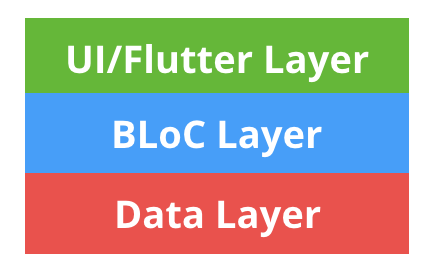
\includegraphics[width=.25\columnwidth]{figures/bloc.png}
    \caption{Standard \gls{bloc} architecture}
    \label{5:fig:bloc}
\end{wrapfigure}

Figure \ref{5:fig:bloc} shows the classic \gls{bloc} structure. Based on this pattern, each page in our application is made up of three main components:
\begin{itemize}
    \setlength{\topsep}{0.5pt}
    \setlength{\itemsep}{0.5pt}
    \setlength{\parsep}{0.5pt}
    \item the \textbf{\acrshort{ui}/\gls{flutter} layer}, also called the \textbf{view}, which acts as a middleman between the user and the \gls{bloc} layer
    \item the \textbf{\gls{bloc} layer}, which we also refer to as the \textbf{\mintinline{dart}{Provider}} or \textbf{service}, contains the actual business logic and communicates with the database
    \item the \textbf{data layer} or the data \textbf{model} contains simple data classes which represent the data that is to be displayed in the \acrshort{ui}, and is provided by the \gls{bloc}
\end{itemize}

For example, the portal page has three main components, which can be observed in appendix \ref{a:uml}, figure \ref{a:fig:uml_portal}. The \textbf{view} manages the \acrshort{ui} and includes both the page listing the websites as well as the form page allowing users to add/modify a website. The \textbf{model} is the \mintinline{dart}{Website} data class and contains all of the relevant fields for a website (e.g., name, link, localized information, path to the icon). The \textbf{service} is a \mintinline{dart}{ChangeNotifierProvider} and is responsible for fetching the data from Firestore and converting it to a list of \mintinline{dart}{Website}s. The service also checks the validity of new data and sends it to the server to be updated.

\subsection{Localization} \label{5:localization}
Thanks to our user study, we know that Romanian and English localization is essential for a large portion of our potential user base (see section \ref{3:language} for the relevant survey results). Therefore, we implemented localization using \gls{flutter}-compatible tools.

The application's localized strings are defined in .ARB (App Resource Bundle)\footnote{https://github.com/google/app-resource-bundle} files, a simple localization resource format based on \gls{json} and introduced by Google. The \textit{Fluter Intl}\footnote{https://plugins.jetbrains.com/plugin/13666-flutter-intl} Android Studio plugin automatically generates \textit{Dart Intl}\footnote{https://pub.dev/packages/intl} boilerplate code which binds the \gls{flutter} application to the translations in the .ARB files.

\section{\acrshort{ci} \& \acrshort{cd}} \label{5:cicd}

\subsection{Testing} \label{5:cicd_testing}

A test-driven approach is necessary for any medium to large project with multiple contributors, to ensure that new changes work as intended and do not break existing features. It has been shown\cite{hilton2009quantitatively} to improve code quality and maintainability significantly.

We decided to use the \mintinline{dart}{flutter_test} library\footnote{https://api.flutter.dev/flutter/flutter\_test/flutter\_test-library.html} to test our application. The \gls{bloc} architecture (described in section \ref{5:separation}) makes it easy to test each individual component. We focused on testing the data and UI layers, since the service layer mostly calls methods from the \mintinline{dart}{flutterfire} plugin\footnote{https://github.com/FirebaseExtended/flutterfire} which connects to Firestore. The Firestore plugin is already heavily tested by its developers and would be complicated to mock. As a result, more than 70\% (fig. \ref{5:fig:codecov}), the application code is being tested through over 200 unit and integration tests. We aim to keep this number above the 60\% threshold.

\begin{figure}[!ht]
    \centering
     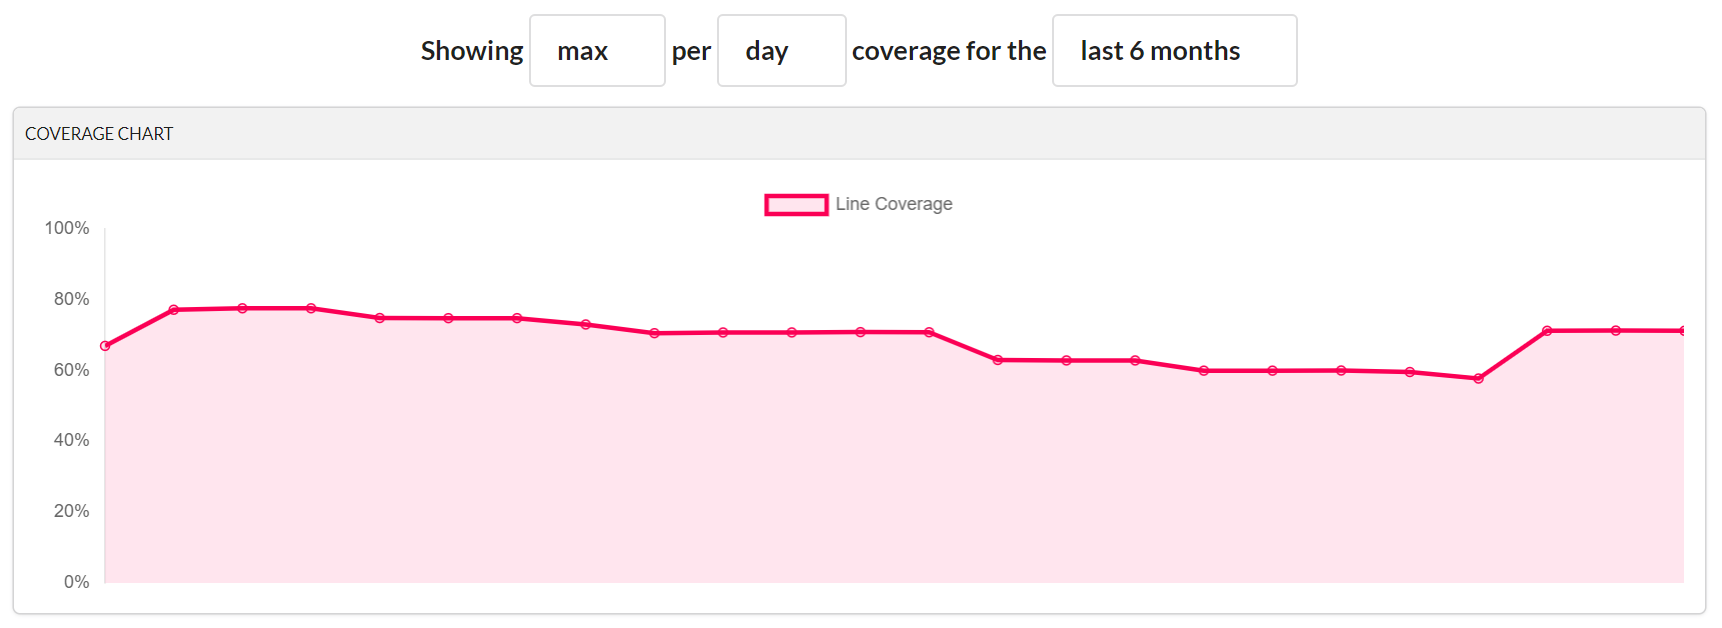
\includegraphics[width=0.95\textwidth]{figures/charts/codecov.png}
     \caption{Application code coverage according to \textit{codecov}}
    \label{5:fig:codecov}
\end{figure}

\subsection{Deployment} \label{5:cicd_deployment}
The application is currently being hosted on the web using two free Firebase domains\footnote{https://acs-upb-mobile.web.app/ and https://acs-upb-mobile.firebaseapp.com/}. Deployment is done through the \mintinline{shell}{firebase deploy} command of the Firebase \acrshort{cli}\footnote{https://firebase.google.com/docs/cli}.

In the future, the mobile application can be published directly onto the App Store and Google Play (see subsection \ref{6:future_publish}) for easy access.

\subsection{GitHub Actions} \label{5:cicd_actions}

The code of the application is public in a GitHub repository\footnote{https://github.com/acs-upb-mobile/acs-upb-mobile/}, which makes it easy for students to contribute by creating an issue or submitting a \acrshort{pr}. GitHub allows setting up an automated testing and deployment pipeline using GitHub Actions\footnote{https://github.com/features/actions/}, which is what we chose to use for our application.

For \acrlong{ci} (\acrshort{ci}), we created a workflow\footnote{https://github.com/acs-upb-mobile/acs-upb-mobile/blob/master/.github/workflows/test.yml} which runs on every push to the repository. It runs all tests (see subsection \ref{5:cicd_testing}) on an Ubuntu virtual machine and sends coverage information to \textit{codecov}\footnote{https://codecov.io/gh/acs-upb-mobile/acs-upb-mobile}. 

For \acrlong{cd} (\acrshort{cd}), we defined a deployment workflow\footnote{https://github.com/acs-upb-mobile/acs-upb-mobile/blob/master/.github/workflows/deploy.yml} which is triggered on the creation of a new tag. It runs all tests and, if they succeed, builds and publishes the web version (see subsection \ref{5:cicd_deployment}) onto the Firebase servers and creates a new release on GitHub containing the built APK for Android devices.